\documentclass[times, 10pt,twocolumn]{article}
\usepackage{dsn}
\usepackage{times}
\usepackage{url}
\usepackage{amsfonts,amsthm,amsmath}

\usepackage{graphicx}
\usepackage[noend]{algorithmic}
\usepackage[boxed]{algorithm}
\algsetup{indent=1.5em}

\newtheorem*{theorem}{Theorem}
\newtheorem*{claim}{Claim}

\newcommand{\sysname}{\textsc{Ajil}}

%-------------------------------------------------------------------------
% take the % away on next line to produce the final camera-ready version
\pagestyle{empty}

%-------------------------------------------------------------------------
\begin{document}

\title{Ajil: Distributed Rate-limiting for Multicast Networks}

\author{Hussam Abu-Libdeh, Ymir Vigfusson, Ken Birman\\
\textit{Department of Computer Science}\\
\textit{Cornell University, Ithaca, NY 14853}\\
\{hussam, vigfusson, ken\}@cs.cornell.edu\\
% For a paper whose authors are all at the same institution,
% omit the following lines up until the closing ``}''.
% Additional authors and addresses can be added with ``\and'',
% just like the second author.
\and
Mahesh Balakrishnan\\
\textit{Microsoft Research Silicon Valley}\\
\textit{Mountain View, CA 94043}\\
maheshba@microsoft.com\\
}

\maketitle
\thispagestyle{empty}

\begin{abstract}
Multicast traffic patterns play a key role in dependable data centers, arising when data is replicated and distributed over multiple machines for fault-tolerance and availability. Such settings involve large numbers of multicast groups as well as multiple senders to each group --- a single system can have hundreds of such multicast channels. Without effective multi-channel rate control, multicast senders cannot determine the right rate to send data at and often transmit to groups as fast as possible. As a result, multicast channels are subject to traffic spikes that can overload individual end-hosts within the data center as well as its communication back-plane. This paper introduces and evaluates Ajil, a distributed rate-limiting protocol for data centers. Ajil enforces a system-wide quota on multicast traffic, and facilitates equitable distribution of this quota across all the multicast channels in the data center.
\end{abstract}



%-------------------------------------------------------------------------
\Section{Introduction}

%Multicast is important for dependable systems --- especially with lots of channels
Multicast is key to building dependable data center systems, enabling the replication of data and functionality over multiple machines for fault-tolerance and availability. In such settings, multicast usage is characterized by large numbers of groups in the system, as well as many different senders transmitting data to each group --- in essence, hundreds of channels between individual senders and groups of receivers.

%without rate control, multicast makes systems less dependable
Unfortunately, multicast rate control in clustered settings is a black art. Senders in a multi-channel setting have no way to determine the right rate to transmit at, and often default to sending data as fast as possible. As a result, systems that use multicast heavily are extremely vulnerable to `black-outs' resulting from disruptive traffic spikes. Multicast channels can interfere with each other as well as other unicast traffic, overloading both end-hosts and the data center switching fabric.

%hence the need for ajil
This paper presents \sysname{}, a distributed rate-limiting protocol for data centers. \sysname{} has three goals: First, it establishes a soft global bandwidth limit on the aggregate multicast traffic in the network. Second, it enables equitable division of this bandwidth limit across multiple groups and senders in the system. Finally, it allows the network administrator to issue an acceptable-use-policy (AUP) specifying the bandwidth limit and what should happen if that limit is exceeded. \sysname{} achieves these goals through a decentralized protocol in which senders use local information representing a partial state of the system to make global decisions on whether they should ramp up or slow down their sending rates. These local estimate are obtained through a broadcast control channel on which receivers periodically and probabilistically transmit information about traffic rates in different groups.

We evaluate a simulation of \sysname{} and demonstrate that it can be used to effectively enforce a soft bandwidth limit in a multi-group setting, and equitably divide this limit across multiple groups as well as the multiple senders in each group. The rest of the paper is organized as follows: we outline the problem statement in Section \ref{sec:probstat}, we describe the operation of the \sysname{} protocol in Section \ref{sec:protocol}, describe the policies it supports in Section \ref{sec:policy} and evaluate a simulation in Section \ref{sec:eval}. After a discussion of related work in Section \ref{sec:related} and future work in Section \ref{sec:future}, we conclude in Section \ref{sec:conclusion}.

%-------------------------------------------------------------------------
\Section{Problem Statement} \label{sec:probstat}

Services in data centers are often provided by collections of nodes running a single application or a suite of applications. To avoid communication black-outs, a network administrator can impose an aggregate multicast limit $L$ in her data center. Assume that $\{n_1 ... n_N\}$ is the set of processes (nodes) in the system, and $\{G_1 ... G_M\}$ be the set of multicast groups in use. Let $r_j(t)$ denote the multicast traffic rate of group $G_j$ at time $t$.

Our goal is to maintain that:
\[ \forall t:\ \sum_{j = 1}^{M} r_j(t) \leq L\]

\subsection{A Trivial Approach}
We can trivially achieve our goal by dividing the allowed multicast bandwidth equally across all the groups and all the senders in each group; that is by hand-wiring that
\begin{eqnarray*}
\forall t, \forall j: r_j(t) &=& \frac{L}{M}
\end{eqnarray*}

However, this quota allotment is hard to achieve in systems where the number of groups and members of each group are only known at run-time. Additionally, equal division of the quota might not be optimal because of unequal multicast demands of different nodes and groups. For this reason, we need a protocol to dynamically assign bandwidth quotas to multicast channels based on demand.

\subsection{Why not TCP?}
TCP is the \textit{de facto} standard for flow and congestion control in practically any kind of network. It uses a simple, decentralized mechanism to ensure that bottleneck bandwidth in a network is equitably distributed across all the unicast flows traversing it.

Clearly, data center operators concerned about flow control could use TCP as the basis of a multicast protocol in the manner of enterprise service bus solutions such as the Java Messaging Service (a popular client-server style of messaging system).  However, in such approaches all messages must pass through the server, which becomes a bottleneck and single point of failure.

Once we accept that direct host-to-host multicast might be preferable, one can still ask whether a direct mapping of the TCP flow control and congestion protocol could solve our multicast problem. Comparing our requirements to TCP sheds light on the nature of a possible solution:\\

\begin{itemize}
\item{TCP is a window-based protocol --- each sender maintains a window of packets sent but not yet acknowledged by the receiver, and only sends more packets when current packets in the window are acknowledged and removed from it. Such a scheme does not work very well for multicast, since it requires each receiver to send back acknowledgments to the sender, an approach that does not scale well with the number of receivers in a group. Instead, we need a protocol that assigns a sending rate to each node for every group it is transmitting to, and varies this rate over time to control the amount of traffic in the system.}
\item{TCP is designed to prevent congestion collapse in networks, and uses packet loss as a signal of congestion. We would like to enforce an administratively defined limit on multicast bandwidth usage, and packet loss does not necessarily occur when this limit is breached; as a result, it is not a valid signal for limit violation.}
\item{Packet loss is a 1-bit signal intrinsically tied to network congestion. To impose an arbitrary bandwidth limit within a data center, we need a more complex signal that tells us when the limit is crossed as well as the senders and groups primary responsible. One such signal is an estimate of the aggregate traffic rate within the system, along with a per-channel breakdown.}
\end{itemize}

Accordingly, we need a solution that assigns sending rates to each multicast channel in the system (i.e, to each sender, for every group it is sending to), and determines this rate locally at each sender by observing a system-wide estimate of traffic. Our assumptions of the operating environment for this solution are as follows:
\begin{itemize}
\item{Nodes are expected to follow the protocol and not behave maliciously. We do assume benign fail-stop faults.}
\item{The clocks of individual nodes in the system are synchronized with each other. In practice, it is possible to achieve sub-millisecond clock synchronization within data centers.}
\item{The data center network is expected to provide a broadcast capability to nodes.}
\end{itemize}


%-------------------------------------------------------------------------
\Section{The Ajil Protocol} \label{sec:protocol}

\newcommand{\E}{\mathbb{E}}

Constructing a strict rate-limiting protocol for multi-party communication requires complete knowledge of all the senders in the system and their sending rates. However this is difficult to achieve without using a centralized server or running a consensus protocol. This is specially the case for systems comprised of multiple non-overlapping groups where nodes do not receive all the multicast messages pushed on the network.

We note that a minor relaxation of the requirements can result in a simple decentralized solution to the rate-limiting problem. Rather than enforcing a strict or `hard' aggregate limit at all times, we will allow occasional and temporary violations, i.e. a `soft' limit. Thus, our goal will be to minimize the frequency of the global limit violations.

An optimal dynamic multi-party rate-limiting protocol uses global information regarding the aggregate traffic rate, and the rates on different channels, and makes decisions to dynamically slow down certain nodes or adjust the bandwidth quota allotted to certain groups. However, The relaxed requirement allows us to build \sysname{} in a decentralized fashion such that nodes can use local information to estimate the global traffic rates and make decisions on which nodes should slow down, and how should the bandwidth quotas be readjusted.

On a high level, a node running the \sysname{} protocol will send multicast messages without restrictions and periodically reevaluate its sending bandwidth quota as to not exceed the global limit. When the limit is exceeded, nodes will apply an administrator-specified \textit{slowdown} policy to reduce their sending rate.

\sysname{} runs in equal-sized time windows, or \textit{epochs}, and has two parts:
\begin{itemize}
\item A \emph{monitor} gathers statistics about multicast use on the network.

\item A \emph{reactor} is activated at the end of each epoch if traffic rates reach a critical threshold of the limit $L$. The reactor reevaluates sending quotas and invokes slowdown policies.
\end{itemize}

Nodes use local estimates obtained by the monitor to evaluate whether the global limit has been exceeded. When the limit is exceeded, a subset of the nodes and groups are designated as a \textit{Reaction Domain} and are required to slow down their sending rates and cut their bandwidth quotas.

\subsection{The Monitor}
Monitors are used to collect local information that estimate the global status of the system. \sysname{} implements the monitor component using a global dedicated broadcast channel. At the end of each epoch, nodes probabilistically broadcast the total amount of traffic that has been sent in the groups they belong to in the previous epoch. This allows all monitoring nodes to track the total multicast use in a decentralized fashion without promiscuously listening for traffic in other groups.

Upon receiving an update $r_j$, the monitor will store it until another update about $G_j$ is received, or for a finite timeout period after which the transmission rate on $G_j$ is assumed to be 0.

The broadcast probability determines the expected accuracy of the local information at each node. The network administrator specifies the expected amount of broadcast traffic to be used for the monitor as a fraction ($c$) of the total amount of multicast used by the rest of the system. At the end of each epoch $t$, a node $n_i \in G_j$ sends a broadcast message with probability $c \cdot \dfrac{r_j(t)}{|G_j|}$.

\begin{claim}
The expected rate of reports published on the broadcast channel is a $c$ fraction of the total multicast traffic in the system.
\end{claim}

\begin{proof}
Assume the multicast traffic rate for group $G_j$ is a constant $r_j = r_j(t)$ for all $t$.
For a fixed a group $G_j$ let
\[
t_{ij} = \left\lbrace \begin{array}{ll} 1 & \textrm{ if node $i$ in $G_j$ sends a report packet} \\
0 & \textrm{ otherwise} \end{array} \right.
\]

Let $t_j = \sum_{i=1}^n t_{ij}$ denote the rate of packets sent to the broadcast channel that deal with group $G_j$. The total rate of packets sent to the broadcast channel is $T = \sum_{j=1}^m t_j$. We have
\begin{eqnarray*}
\E[T] &=& \sum_{j=1}^m \sum_{i=1}^n \E[t_{ij}] \\
&=& \sum_{j=1}^m \sum_{i \in G_j} c \frac{r_j}{|G_j|}  \\
&=& c \sum_{j=1}^m r_j,
\end{eqnarray*}
by the linearity of expectation, which proves the claim.
\end{proof}


\subsubsection{Smoothed Rate Aggregation}
To filter out the effects of spikey sending rates, monitors can keep track of an exponential moving average (EMA) of the communication rates of other nodes and groups. More specifically, let $0 < \gamma \leq 1$ be the \textit{smoothing factor} for the exponential moving average function. Each node records
\[ r_j(t) = \gamma \cdot o_j(t) + (1 - \gamma) \cdot r_j(t-1) \]

where $o_j(t)$ is the observed communication rate of $G_j$ during epoch $t$. Notice that by setting $\gamma = 1$ we will have $r_j(t) = o_j(t)$.


\subsection{The Reactor}
Nodes activate their reactor component when aggregate traffic rates reach a critical threshold of the limit $L$. Each node uses its local estimates to independently compute whether it is part of the reaction domain or not. Nodes in the reaction domain will apply a slowdown policy adjusting the bandwidth quotas for subsequent epochs.

\subsubsection*{Reaction Domains}
A reaction domain is defined as the top $\beta$ highest traffic nodes in the top $\alpha$ highest traffic groups. For this we explicitly define $0 < \alpha \leq 1$ to be the fraction of the highest traffic groups to be included in the domain, and $0 < \beta \leq 1$ to be the fraction of the highest traffic nodes to be included in the domain.

At the end of epoch $t$, node $n_i$ in group $G_j$ uses the information supplied by the monitor to compute the reaction domain. $n_i$ determines if $G_j$ is in the reaction domain by computing if:

\begin{center}
\verb|rank of| $G_j$ \verb|by traffic| $\leq \lceil \alpha M \rceil$\\
(i.e. if $G_j$ is one of the top $\alpha$ groups)
\end{center}

If so, $n_i$ checks if:
\begin{center}
\verb|rank of| $n_i$ \verb|by traffic in| $G_j \leq \lceil \beta |G_j| \rceil$\\
(i.e. if $n_j$ is one of the top $\beta$ senders in group $G_j$)
\end{center}

If so, $n_i$ is in the reaction domain and applies the slowdown policy in subsequent epochs.

\begin{figure}[t]
 \centering
 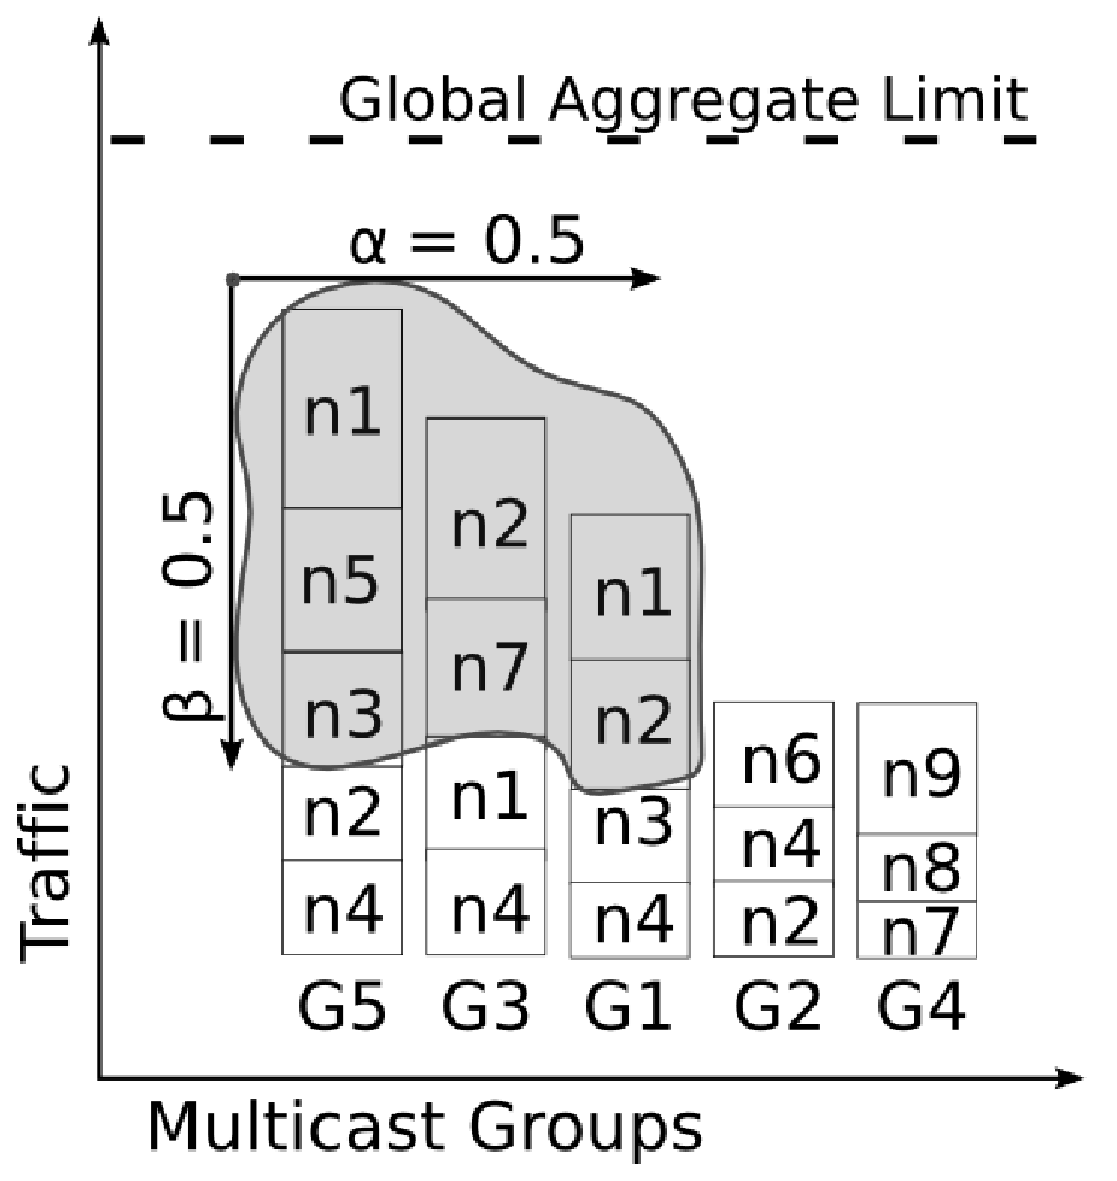
\includegraphics[scale=0.4]{figures/reaction-domain-bubble-gray.eps}
 \caption{An illustration of a reaction domain configured with parameters $\alpha=0.5, \beta=0.5$. The reaction domain (shaded area) encompasses the top $\beta$ senders in the top sending $\alpha$ groups.}
 \label{ill:reaction-domain}
\end{figure}

Figure ~\ref{ill:reaction-domain} shows an illustration of a reaction domain computed in an instance with five sending groups. The groups are sorted decreasingly by traffic from left to right, and the senders within each group are sorted decreasingly by traffic in that group from top to bottom. The reaction domain then is computed by taking the top $\beta$ senders in the first $\alpha$ groups. Notice that this construction means that the reaction domain can change in different epochs. Additionally, the use of local estimates implies that different nodes might have different estimates for the reaction domain in this epoch. 



%-------------------------------------------------------------------------
\Section{Policy} \label{sec:policy}

\begin{algorithm}[t]
Monitor:
\begin{algorithmic}[1]
\STATE listen for incoming traffic broadcasts
\FORALL {$G_j$ \textbf{in} joined groups}
   \STATE {$r_j \gets$ locally-seen traffic rate}
   \IF { rand() $\leq c \cdot \frac{r_j}{|G_j|}$ }
         \STATE \verb|broadcast|($r_j$)
   \ENDIF
\ENDFOR
\end{algorithmic}

\medskip
Reactor:
\begin{algorithmic}[1]
\STATE sort groups by traffic
\IF {$G_j$'s sorted index $\leq \lceil \alpha \cdot M \rceil$}
   \STATE sort members of $G_j$ by traffic
   \IF {my sorted index $\leq \lceil \beta \cdot |G_j| \rceil$}
      \STATE multiplier $\gets 1$
      \STATE apply \verb|slowdown()|
   \ENDIF
\ENDIF
\end{algorithmic}

\medskip
Slowdown:
\begin{algorithmic}[1]
\IF {total traffic using multiplier/2 $\leq L$}
   \STATE multiplier $\gets$ multiplier/2
\ENDIF

\STATE quota $\gets$ \verb|slowdown_policy| * multiplier/2

\IF {multiplier is sufficiently small}
   \STATE stop slowing down
\ENDIF
\end{algorithmic}
\medskip

\floatname{algorithm}{Pseudocode}
\label{pcode}
\caption{\hbox{\tenhv\noindent High-level pseudocode of \sysname{}.} }
\end{algorithm}

The \sysname{} protocol allows the network administrator to specify an acceptable-use-policy (AUP) to govern multicast traffic in her network. The AUP is specified in terms of the protocol's parameters and a slowdown policy to be implemented when the aggregate rate-limit is exceeded.

\subsection{Protocol Parameters}
The network administrator specifies values for the following parameters governing the protocol's performance:
\begin{itemize}
\item The aggregate rate-limit \(\mbox{\boldmath $L$}\).
\item An epoch size (window length). This will determine how often is the monitor checked and how quickly does the protocol react to aggregate limit violations.
\item The monitor broadcast fraction \(\mbox{\boldmath $c$}\) set to a value between 0 and 1. As discussed previously, this governs the frequency of traffic reports sent by the monitor on the broadcast channel. Traffic reports for group $G_j$ are sent at a rate proportional to $c \cdot r_j$. For example, $c=0.01$ implies that for every 100 packets sent on a group, a single traffic report will be sent in expectation.
\item Reaction domain parameters:
	\begin{itemize}
	\item \(\mbox{\boldmath $\alpha$}\): the fraction of the top-sending groups that will be included in the reaction domain. This parameter should be given a value between 0 and 1, where 1 indicates all the groups and 0 is specially reserved for the single highest sending group.
	\item \(\mbox{\boldmath $\beta$}\): the fraction of the top-sending nodes within the top-sending groups to be included in the reaction domain. This parameter should be set to a value between 0 and 1 as well with the same meaning as before.
	\end{itemize}
\end{itemize}

\subsection{Slowdown Policy}
The network administrator also specifies a \textit{slowdown} policy governing how a violation of the aggregate limit is handled. The slowdown policy is implemented by the nodes that are in the current reaction domain. A slowdown policy can be defined as any number of things for example:

\begin{itemize}
\item \textbf{Flat Tax:} each node slows its sending rate by some constant KBps.
\item \textbf{Local Percentage:} each nodes slows down by some fixed percentage.
\item \textbf{Global Percentage:} each node slows down proportional to the global excess over the aggregate limit.
\end{itemize}

Our evaluation showed that 'fairness' is best achieved when nodes are slowed down proportionally to their transmission rate following the global percentage scheme above.

The actual meaning of a 'slowdown' is left for implementation and can be part of the policy itself. For example, a slowdown can be implemented as any of the following:
\begin{itemize}
\item \emph{Drop} packets --- This policy suits applications that do not require 100\% reliability from the transport layer, either running their own application-level reliability protocols or sending data that is intrinsically tolerant of some loss.
\item \emph{Delay} each outgoing packet --- For applications that require a reliable transport layer, \sysname{} can delay packets at send-side buffers instead of dropping them.
\end{itemize}

Changes made to the policy parameters by an administrator are propagated by broadcasting on the shared channel.

\subsection{Slowdown Policy Application}
\sysname{}'s rate control policies are a superset of TCP's AIMD curve; with the local and global percentage policies, \sysname{} supports an MIMD (Multiplicative Increase Multiplicative Decrease) curve, whereas with the flat tax policy, it supports an AIAD policy (Arithmetic Decrease Arithmetic Increase).

For MIMD policies, a ``slowdown multiplier'' is initialized to 1 when the slowdown is first initiated. In each epoch while the slowdown policy is activated, the bandwidth quota is cut at minimum by a 'multiplier factor' of the amount dictated by the policy. Opportunistically, nodes check whether cutting the quota by half the multiplier factor of the amount dictated by policy will not exceed the global bandwidth limit according to the information gathered by the node's monitor. If the latter is the case, then that option is followed, and the multiplier is set to half its value for the subsequent epochs. Otherwise, the quota is cut down by the first amount and the multiplier is kept at its current value.

For example, in the first epoch of a slowdown, the node tests whether it should slowdown by the full amount dictated by policy or half of it. If slowing down by half the amount is possible, then the multiplier is set to 0.5 and later epochs test whether they could minimize that deduction any further. With this mechanism, nodes stop slowing down when the multiplier reaches a sufficiently low value.

With this we have a complete description of \sysname{}. Pseudocode 1 provides a high level summary of our protocol. 



%-------------------------------------------------------------------------
\Section{Simulation and Experimental Results	} \label{sec:eval}

\begin{figure*}[ht]
 \centering
 %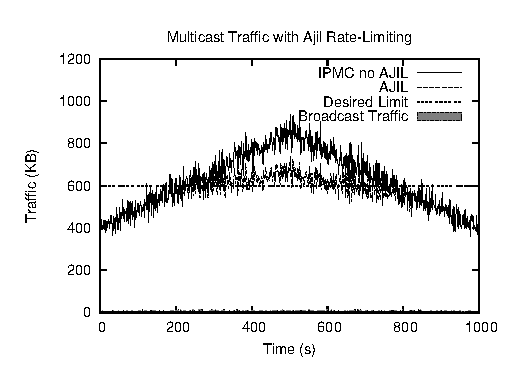
\includegraphics[scale=1]{figures/evaluation/rate-limiting/ajil-peek.eps}
 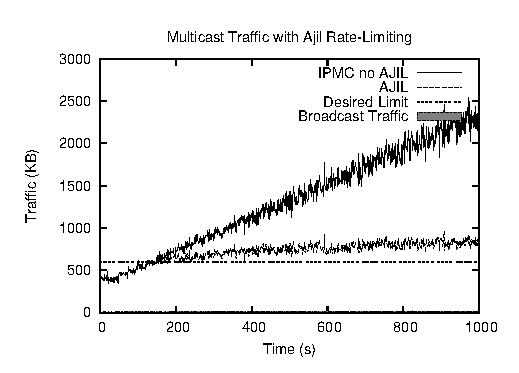
\includegraphics[scale=1]{figures/evaluation/rate-limiting/ajil-linear.eps}
 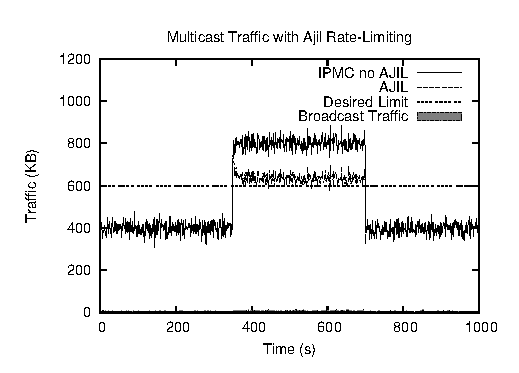
\includegraphics[scale=1]{figures/evaluation/rate-limiting/ajil-square.eps}
 \caption{Multicast traffic rate-limited by \sysname{} under different communication patterns.}
 \label{fig:rate-limiting}
\end{figure*}

In this section, we evaluate the \sysname{} protocol by simulation. The simulator uses the previously described algorithm and some simple acceptable use policies.

Our evaluation has multiple goals. We first test our protocol's rate-limiting capabilities with a couple of multicast traffic patterns. We then evaluate the effects of manipulating the protocol's parameters as part of the AUP. Additionally we test how the slowdown policy is being applied across groups and individual communication channels. Finally we test two simple administrator-defined slowdown policies and highlight their differing effects.

\subsection{Setup}
We based the setup of our nodes and multicast groups on a previously-acquired multicast trace of an IBM Websphere \cite{websphere} deployment. That trace showed an internal publish-subscribe component of Websphere using over 6,600 multicast groups averaging 10 members per group.

Our simulator generates multiple communication patterns to reflect different data center deployments. During initialization, nodes subscribe to the various multicast groups uniformly and read-in a program file dictating the number and size of messages to be sent during each epoch. This file simulates the application load. From the perspective of our protocol, during each epoch the application sends multicast requests down to the protocol which puts them down on the network as long as its current quota has not been exceeded. At the end of each epoch, nodes reevaluate their sending quota for every multicast channel on each group. We have assumed a model in which sending packets up to the current quota and then dropping the rest is acceptable.

\subsection{Rate-Limiting}
Figure ~\ref{fig:rate-limiting} shows the aggregate multicast traffic of a network with a soft rate-limit of 600 KBps. The figure depicts two communication patterns. Both networks start with traffic rates of about 400KBps. The first graph on the left shows a continuous gradual increase in raw IP Multicast traffic in the unmanaged case. When \sysname{} is used to manage multicast, the traffic increase is severely limited. The managed multcast rate does not drop below the desired limit in the first graph because \sysname{} is reactive in nature, and thus the bandwidth is adjusted in every epoch reflecting the state as it was in previous epochs.

%The first graph on the left shows a gradual increase of the communication rate to over 800KBps and then a graduate decline. This pattern arises in situations where ``flash'' multicast groups are setup dynamically to execute certain jobs and are then deleted. A gradual incline/decline is the result of inter-dependencies between the jobs being executed. So an increasing number of ``flash groups'' could be set up to process a set of jobs, and as soon as the root job has been executed all the dependencies start to finalize and terminate. We know of at least one widely deployed commercial data center application using this pattern.

The second graph on the right represents a more common case. The aggregate traffic in the network is steady at around 400KBps when suddenly an event, or a faulty process, triggers high multicast rates which push the aggregate traffic over the set limit. As soon as that event terminates the traffic rates go back to normal.

Both graphs in figure ~\ref{fig:rate-limiting} show that \sysname{} does not affect the multicast rates as long as they do not exceed the limit. Once the limit is exceeded, \sysname{} minimizes the excess. Notice that the lower peeks above the limit line in both graphs are those of rate-limited multicast. Even though the raw traffic rates exceed the limit by over 20\%, by using \sysname{} this excess is sharply reduced.

In this experiment we set the protocol parameters to: $\alpha=0.5, \beta=0.25$, and a monitor broadcast factor $c=0.01$. Notice that in both graphs the aggregate broadcast traffic used by all the monitors is reported at the bottom and is minimal in comparison to the aggregate multicast traffic in use.

\begin{figure}[t]
 \centering
 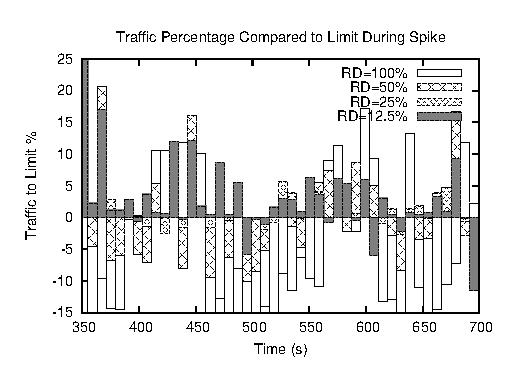
\includegraphics[scale=1]{figures/evaluation/rd/reaction-waves.eps}
 \caption{The oscillation effect in different reaction domain sizes.}
 \label{fig:varied-rd}
\end{figure}

\subsection{Reaction Domain Size}
We tested various sizes for the reaction domain trying to determine an optimal selection. We note that the effects of the size of the reaction domain are largely dependent on the slowdown policy specified by the administrator. For example, using a reaction domain encompassing all the nodes and a slowdown policy that scales back the quotas for all the senders by a fixed percentage has the effect of scaling down the entire network when the global limit is violated. On the other hand, if the administrator wishes to balance the multicast bandwidth consumption between the nodes, she might opt for choosing smaller reaction domains and implementing a slowdown policy that scales back the top senders to either a fixed upper-limit or by a fraction of their previous sending quota.

\begin{figure*}[t]
 \centering
 \includegraphics[scale=1]{figures/evaluation/staleness/excess-during.eps}
 \includegraphics[scale=1]{figures/evaluation/staleness/utility-after.eps}
 \caption{The effects of monitor staleness.}
 \label{fig:monitor-staleness}
\end{figure*}

However we observe that regardless of the slowdown policy in use, a certain pattern emerges. Since nodes rely on data of previous epochs to estimate the global traffic for subsequent epochs, it is often the case that when a group of nodes slow down in an epoch, the aggregate traffic in the subsequent epoch falls below the global limit. This can be either because of the slowdown mechanism being applied, or because other senders that were not part of the reaction domain have reduced their rates due to a reduced demand by the application. In that case, all the nodes that slowed down in the previous epoch will decide to increase their quota in the next epoch. This will result in exceeding the limit in the next epoch. This pattern of overshooting and undershooting can continue for multiple epochs. This results in an oscillatory pattern of traffic surging above or dropping below the limit.

This oscillation, however, dampens with time. This is caused by several factors: first, when nodes increase their quota after being slowed down, they do that in a multiplicative way, and the quota increase amounts to 50\% of the quota reduction implemented in the previous epoch. In addition to that, nodes that are currently applying a slowdown policy do not decrease their quota after they have increased it. This means that the multiplicative increases can not be rolled back after they have been issued. So in each epoch, the percentage by which a node in the reaction domain can speed up and slow down is monotonically decreasing. Thus this oscillatory behavior dampens with time.

However, the speed of this dampening depends on the size of the reaction domain. In large reaction domains, the oscillation is bigger in magnitude because there are more nodes that can potentially slowdown or speed up after each epoch. Figure ~\ref{fig:varied-rd} shows the oscillatory behavior of different reaction domains. In this experiment we fixed the communication pattern, and the network setup while varying the size of the reaction domain. We set the $(\alpha, \beta)$ parameters to: (1,1) which is 100\% of the nodes, and (1, 0.5), (0.5, 0.5), (0.5, 0.25) which roughly correspond to 50\%, 25\% and 12.5\% of all the nodes in a setting were the nodes are equally distributed among all the groups. Figure ~\ref{fig:varied-rd} plots the percentage of the difference between aggregate traffic rates and the imposed limit. So a value of +5\% denotes exceeding the limit by 5\%, and -5\% denotes sending 5\% below the limit. As illustrated by figure ~\ref{fig:varied-rd}, smaller reaction domains experience smaller-magnitude oscillation as expected.




\subsection{Monitor Staleness}

As explained previously, nodes rely on the monitor component of the protocol to gather data about the sending patterns of other nodes and other groups in the system. Nodes then use that collected information to make local decisions on whether to invoke the reactor and apply the slowdown policy or not. Monitors use a broadcast channel and probabilistically publish the traffic rates of their nodes. In this experiment we manipulated the monitor broadcast frequency ($c$) to measure its effect on the responsiveness of the protocol. A low broadcast frequency implies a lower probability for a particular monitor to publish its most recent information, which also implies that nodes often have to rely on old stale data when reevaluating the sending quota between epochs. This staleness implies a slower reaction to a limit violation, and a slower speedup after the violation has been removed.

\begin{figure*}[t]
 \centering
 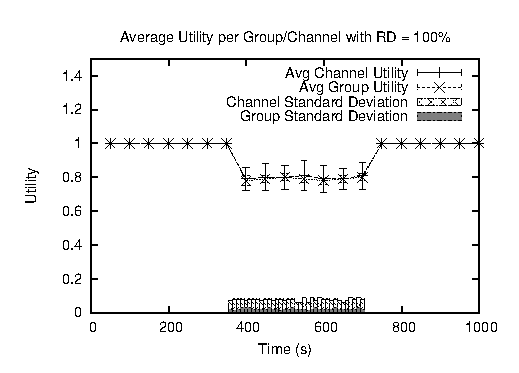
\includegraphics[scale=1]{figures/evaluation/fairness/utility-rd1.eps}
 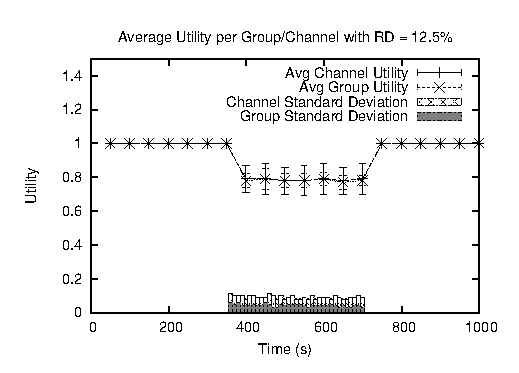
\includegraphics[scale=1]{figures/evaluation/fairness/utility-rd.125.eps}
 \caption{The average ratio of the allotted quota to the requested quota of each group and channel.}
 \label{fig:utility}
\end{figure*}

Figure ~\ref{fig:monitor-staleness} shows the affect of the broadcast frequency $c$ on the responsiveness of the protocol. We used the square wave traffic pattern as shown in the right graph of figure ~\ref{fig:rate-limiting} where the limit is being exceeded during the time interval [350, 700]. We measured the responsiveness of the system under two broadcast frequencies: $c=0.01$ which has been used for the rest of the experiments thus far, and a smaller $c=0.001$. The first graph on the left in figure ~\ref{fig:monitor-staleness} shows the percentage by which \sysname{} overshoots the limit during the time the limit is being exceeded. As expected, with a smaller broadcast frequency, nodes are less aware of the changes in the sending patterns of other nodes, and thus their bandwidth quotas have not been limited to avoid the excess. This results in the protocol overshooting beyond the limit by a larger fraction than that experienced by the larger $c$ value.

The broadcast frequency also affects the responsiveness of the protocol in recovering from a limit violation. The second part on the right of figure ~\ref{fig:monitor-staleness} shows how quickly the protocol recovers from the limit violation. The graph shows the total allotted quota as a percentage of the requested quota after the limit violation has ended. In an optimal case, the utility should be 100\% immediately after time $t=700$, since that is when the spike ends as shown in figure ~\ref{fig:rate-limiting}. As expected, we see that a higher broadcast frequency results in a faster recovery from a limit violation, because nodes are more aware of the reduced sending rates of other nodes and thus expand their own quotas.

\subsection{Fairness and Utility}

We achieved rate-limiting by slowing down a subset of the senders in the system. However, in the worst case scenario this could result in a subset of the senders being completely denied multicast access while other nodes receive the full bandwidth quota that they ask for. We define \textit{utility} as the percentage of the requested bandwidth that is ratified by the sending quota of a node or group. We get a sense of the 'fairness' of the protocol by analyzing the variance of the utilities on each multicast group: a high variance implies an uneven distribution of utilities among the nodes. We can also measure the utility of each channel (sender on a group). Intuitively, the fairness of the protocol depends on the administrator's policy and the protocol parameters.

Figure ~\ref{fig:utility} shows the utility per channel and per group for the same network under two different policies. In both cases the slowdown policy has been set to slowdown the nodes in the reaction domain by a percentage that is proportional to the fraction of traffic being sent in excess above the global rate limit. However, in the first graph on the left the reaction domain has been set to include all the nodes and all the senders (i.e. the entire network scales back when the limit is violated). Meanwhile, the second graph on the left uses the 12.5\% reaction domain ($\alpha=0.5, \beta=0.25$) that we have seen before.

As expected, the variance of the group utility is much lower with the reaction domain is larger because more groups are being scaled back. In both cases the variance of the channels utility is larger than the variance of the groups utility. This is because the uniform distribution of nodes to groups results in having the bandwidth demands for groups be very comparable. However, each channel represents the multicast demands of a single node on a single group. So channels are much more varied by definition. This means that when channels with low demands are slowed down their nodes will increase and regain their quotas quickly because they do not contribute much to the overall aggregate traffic and will thus find the capacity to increase their quotas. This means that low demand channels can achieve 100\% utility much easier than large demand channels. This heterogeneity between the channels demands results in a more varied utility for them, which explains the higher variance we see in figure ~\ref{fig:utility} for channels when compared to groups.


\subsection{Policy}
In the experiments we ran so far, we have used a single slowdown policy. The slowdown mechanism involved reducing the quota of all the nodes in the reaction domain by the same fraction as the excess in multicast traffic above the aggregate limit. However, as eluded to before, the choice of policy has direct impact on the performance of the protocol.

\begin{figure*}[t]
 \centering
 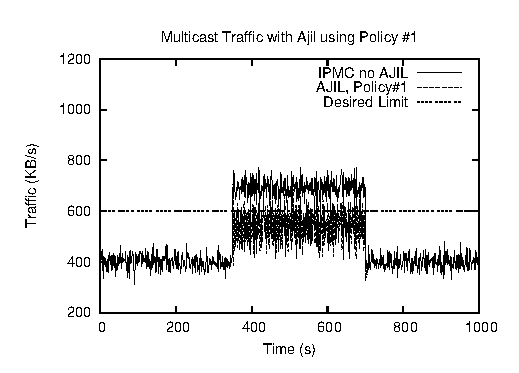
\includegraphics{figures/evaluation/policy/ajil-policy1.eps}
 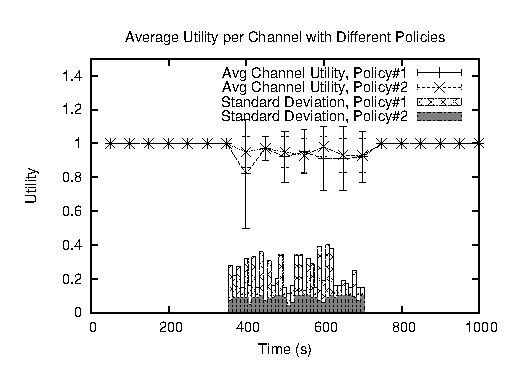
\includegraphics{figures/evaluation/policy/channels-utility.eps}
 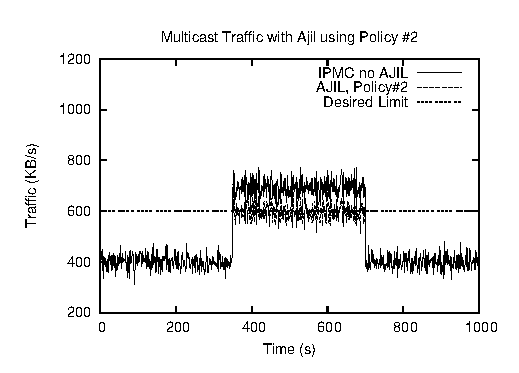
\includegraphics{figures/evaluation/policy/ajil-policy2.eps}
 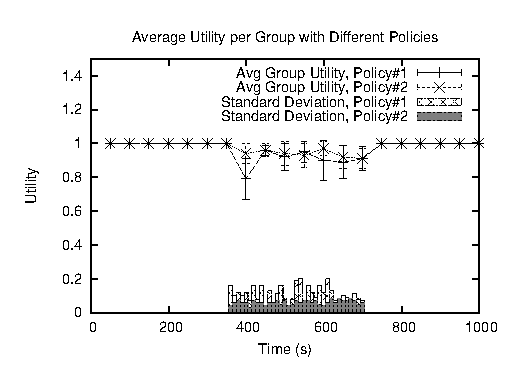
\includegraphics{figures/evaluation/policy/groups-utility.eps}
 \caption{The top left part shows a naive slowdown policy resulting in unstable traffic when the multicast demand exceeds the global limit. The bottom left part shows a more stable slowdown policy producing a more stable traffic pattern. The right side shows the effects of the two policies on group and channel utilities.}
 \label{fig:policy}
\end{figure*}

In this experiment we implemented another slowdown policy with a strict and naive slowdown mechanism dictating that nodes in the reaction domain set their quotas to 0 in the first epoch in which they are in the reaction domain, and then multiplicatively increase their quota (by multiplicatively decreasing the slowdown amount by 50\% if possible). As figure ~\ref{fig:policy} shows, although this policy quickly reduces the violating traffic, it does not result in fairly distributed group and channel utilities.

The top left part of figure ~\ref{fig:policy} shows the aggregate traffic as a result of running the naive policy (\#1) as compared with running our old, fraction-based, policy (\#2) in the bottom left. Although the naive policy cuts excess traffic more quickly than the old policy, it results in extreme fluctuation of traffic rates near the limit. This happens because as soon as the global traffic reaches the limit, a bunch of nodes stop sending immediately causing a quick dip in the aggregate traffic. Following that, the nodes start sending again and the pattern repeats.

The right side of figure ~\ref{fig:policy} shows the difference in channel and group utilities between the two policies. On the top we see that the per-channel utilities are much more variant under the naive policy. This follows intuition because channels are repeatedly being closed (quota set to 0) and then reopened. A similar effect is seen for the group utilities at the bottom right part of the figure.


%-------------------------------------------------------------------------
\Section{Related Work} \label{sec:related}

A large body of work examines multicast flow control within single groups on the wide area network. A primary challenge in WAN settings is the heterogeneous nature of receiver network capacities \cite{gau2002mfc}. One important approach used specifically for video or audio multicast is \textit{layering} \cite{Mccanne96layered, bhattacharyya1998emf, vicisano98tlc}, where a single multicast channel is divided up into multiple separate groups, each transmitting a stripe of the data; receivers can join a subset of these groups to receive data at a specific resolution. \sysname{} differs from these schemes in three important ways --- it's designed for data centers and not a heterogeneous WAN, it is aimed at data that cannot be sent at multiple resolutions, and it looks to enforce a maximum data rate across multiple groups and senders.

In clustered settings, flow control is commonly found as a component in group communication systems --- for example, in the Isis \cite{birman1993pga}, Horus \cite{vanrenesse1996hfg} and Totem \cite{moser1996tft} systems. The challenge for these protocols is usually to avoid overloading individual receivers in the group. In contrast to these approaches, \sysname{} seeks to limit aggregate multicast usage across multiple groups within a data center.

In the absence of effective rate control mechanisms that can prevent packet loss, data center applications often resort to sending packets as fast as possible and using reliability protocols to recover lost packets \cite{ricochet}. Variants of reliability protocols such as SRM \cite{sallysrm} are used in current data centers.

\section{Future Work} \label{sec:future}

Our immediate focus is on implementing \sysname{} and evaluating it on a real data center testbed. We are looking to obtain additional real traces of data center multicast usage --- group sizes, numbers of senders, and traffic rates --- in order to better understand how \sysname{} behaves in different data center deployments.

An important avenue of future research involves prioritizing certain channels over others; for example, in an e-commerce setting, we would prefer slowing down a group used by a background maintenance application instead of a high-value group dedicated to credit card transactions. Additionally, we would like to explore the possibility of having \sysname{} enforce `hard' limits on bandwidth usage that should never be violated, as opposed to soft limits that can be violated momentarily.

\sysname{} was developed in the context of a system called Dr.Multicast \cite{mcmd}, aimed at making data center multicast more manageable by providing access control and resource allocation for groups. We aim to integrate the \sysname{} implementation into Dr.Multicast as a rate control solution for enforcing system-wide bandwidth limits.


%-------------------------------------------------------------------------
\Section{Conclusion} \label{sec:conclusion}

Multicast can play a crucial role in speeding up dependable applications; yet, it is largely underutilized in modern data centers due to the absence of effective mechanisms for limiting its impact on the network. \sysname{} is a simple, distributed rate limiting protocol that allows data center administrators to place a global bandwidth limit on multicast traffic. Furthermore, \sysname{} enables equitable distribution of bandwidth quotas across the multiple groups within the data center, as well as the different senders to each group. Importantly, \sysname{} is completely decentralized, using local estimates of global state to provide a robust communication primitive with no single point of failure.
	
%-------------------------------------------------------------------------
\bibliographystyle{dsn}
\bibliography{ajil}

\end{document}

